\documentclass{article}

\usepackage{geometry}
\geometry{a4paper}
\setlength{\parindent}{10mm}
\setlength{\parskip}{0.9em}
\def\baselinestretch{1.5}

\usepackage[spanish]{babel}
\renewcommand {\spanishtablename}{Tabla}
\usepackage[utf8]{inputenc}
\usepackage{graphicx}
\usepackage{caption} 
\usepackage{amsmath, amsthm, amsfonts}
\usepackage{enumerate} 
\usepackage{fancyhdr}
\usepackage{anysize} 
\usepackage[usenames]{color}
\usepackage{booktabs}

\pagestyle{fancy}

\chead{}
\lhead{} 
\rhead{}
\lfoot{\it }
\cfoot{}
\rfoot{\thepage}

\title{
\centering
Modelos Probabilistas Aplicados \\
Johanna Bolaños Zúñiga \\
Matricula: 1883900\\
Tarea 3
}

\date{}

\begin{document}
\maketitle

\section{Libro Seleccionado --- \textit{The Scarlet Letter}}

En el presente trabajo se continua con el libro \textit{The Scarlet Letter}, el cual se encuentra disponible de manera gratuita en \textit{Project Gutenberg} \cite{libro}. En esta ocasión, se analizó el tipo de distribuciones discretas que podrían estar contenidas en el escrito mediante el programa R versión 4.0.2 \cite{r}. El código en R se encuentra en el repositorio de GitHub \cite{github}.

\section{Distribuciones}
Para el análisis de las distribuciones, se consideró reflejar cómo se comporta la longitud de las palabras presentes en el libro y la cantidad de palabras en cada párrafo. Para este último criterio, se determinó usar párrafos que contienen más de 9 palabras, ya que el título más largo contiene 9 palabras.

De acuerdo a la figura \ref{largoPalabras}, se puede observar que la distribución de la longitud de cada palabra se asemeja a una distribución binomial. Mientras que, en la figura  \ref{palParrafos} correspondiente a la cantidad de palabras por párrafos, es similar a la geométrica.



\begin{figure}
\centering
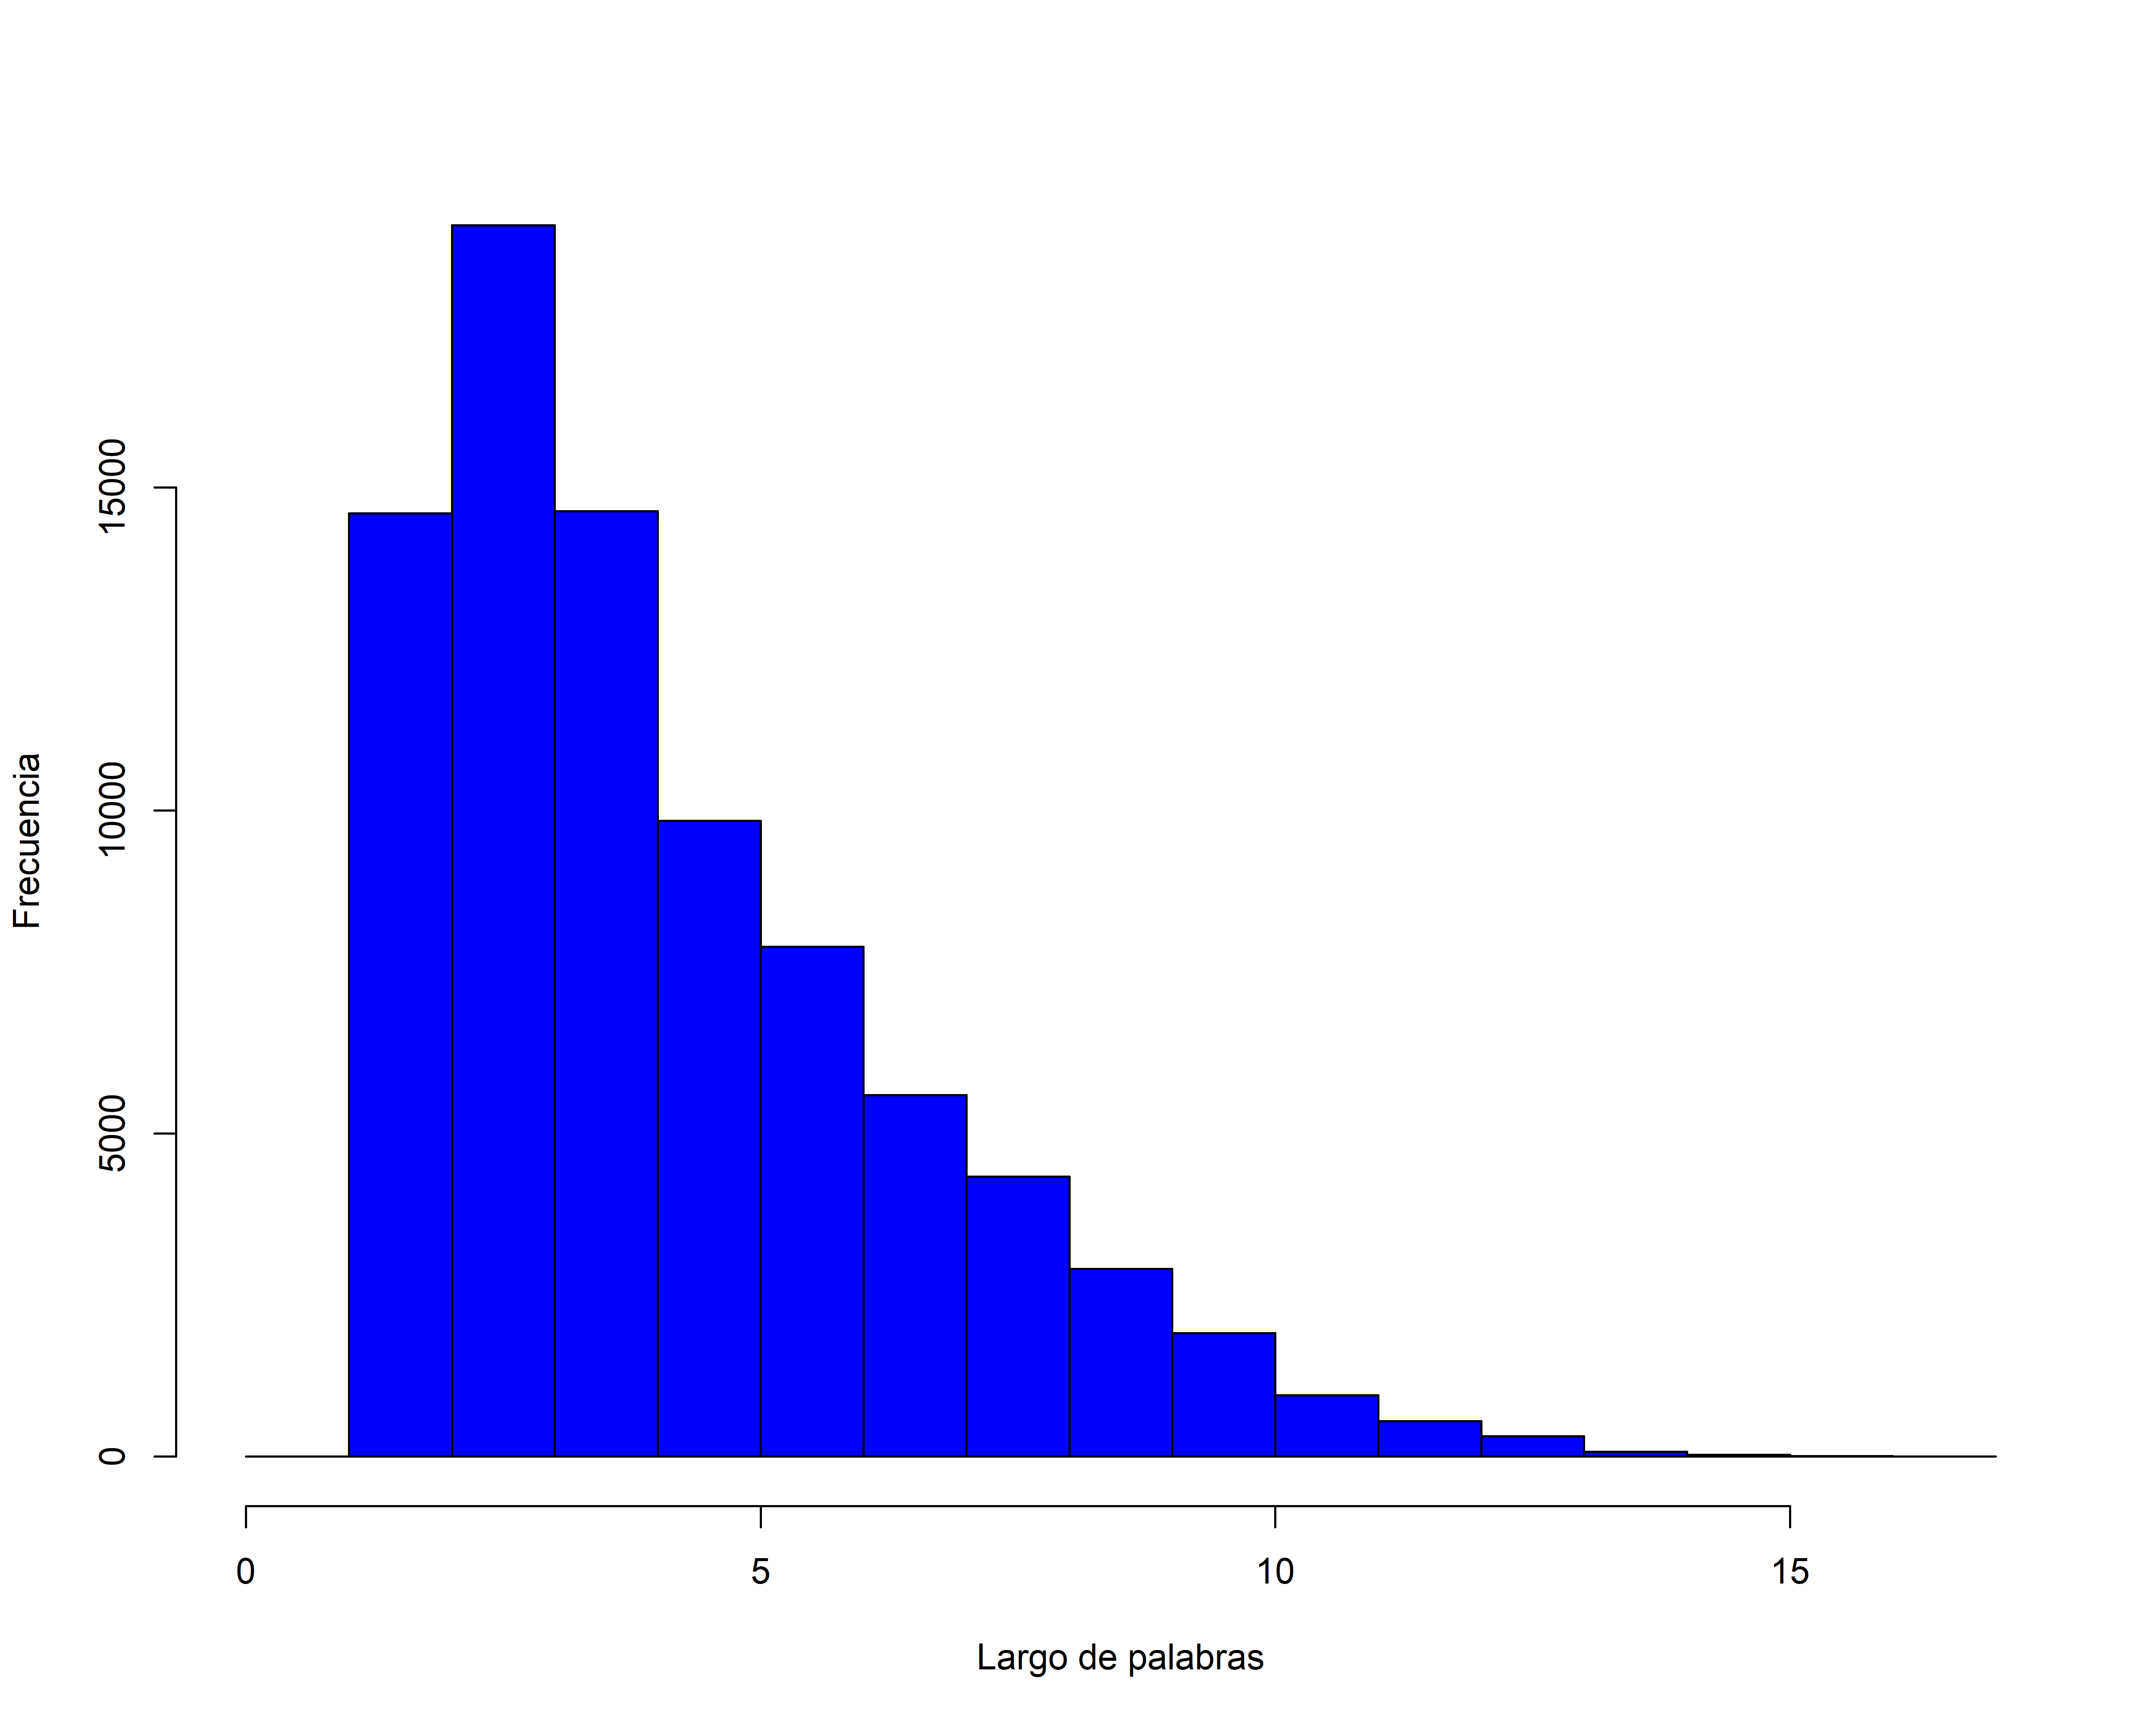
\includegraphics[scale=0.5]{Figures/largoPalabras.png}
\caption{Distribución de la longitud de las palabras usadas en el libro}
\label{largoPalabras}
\end{figure}



\begin{figure}
\centering
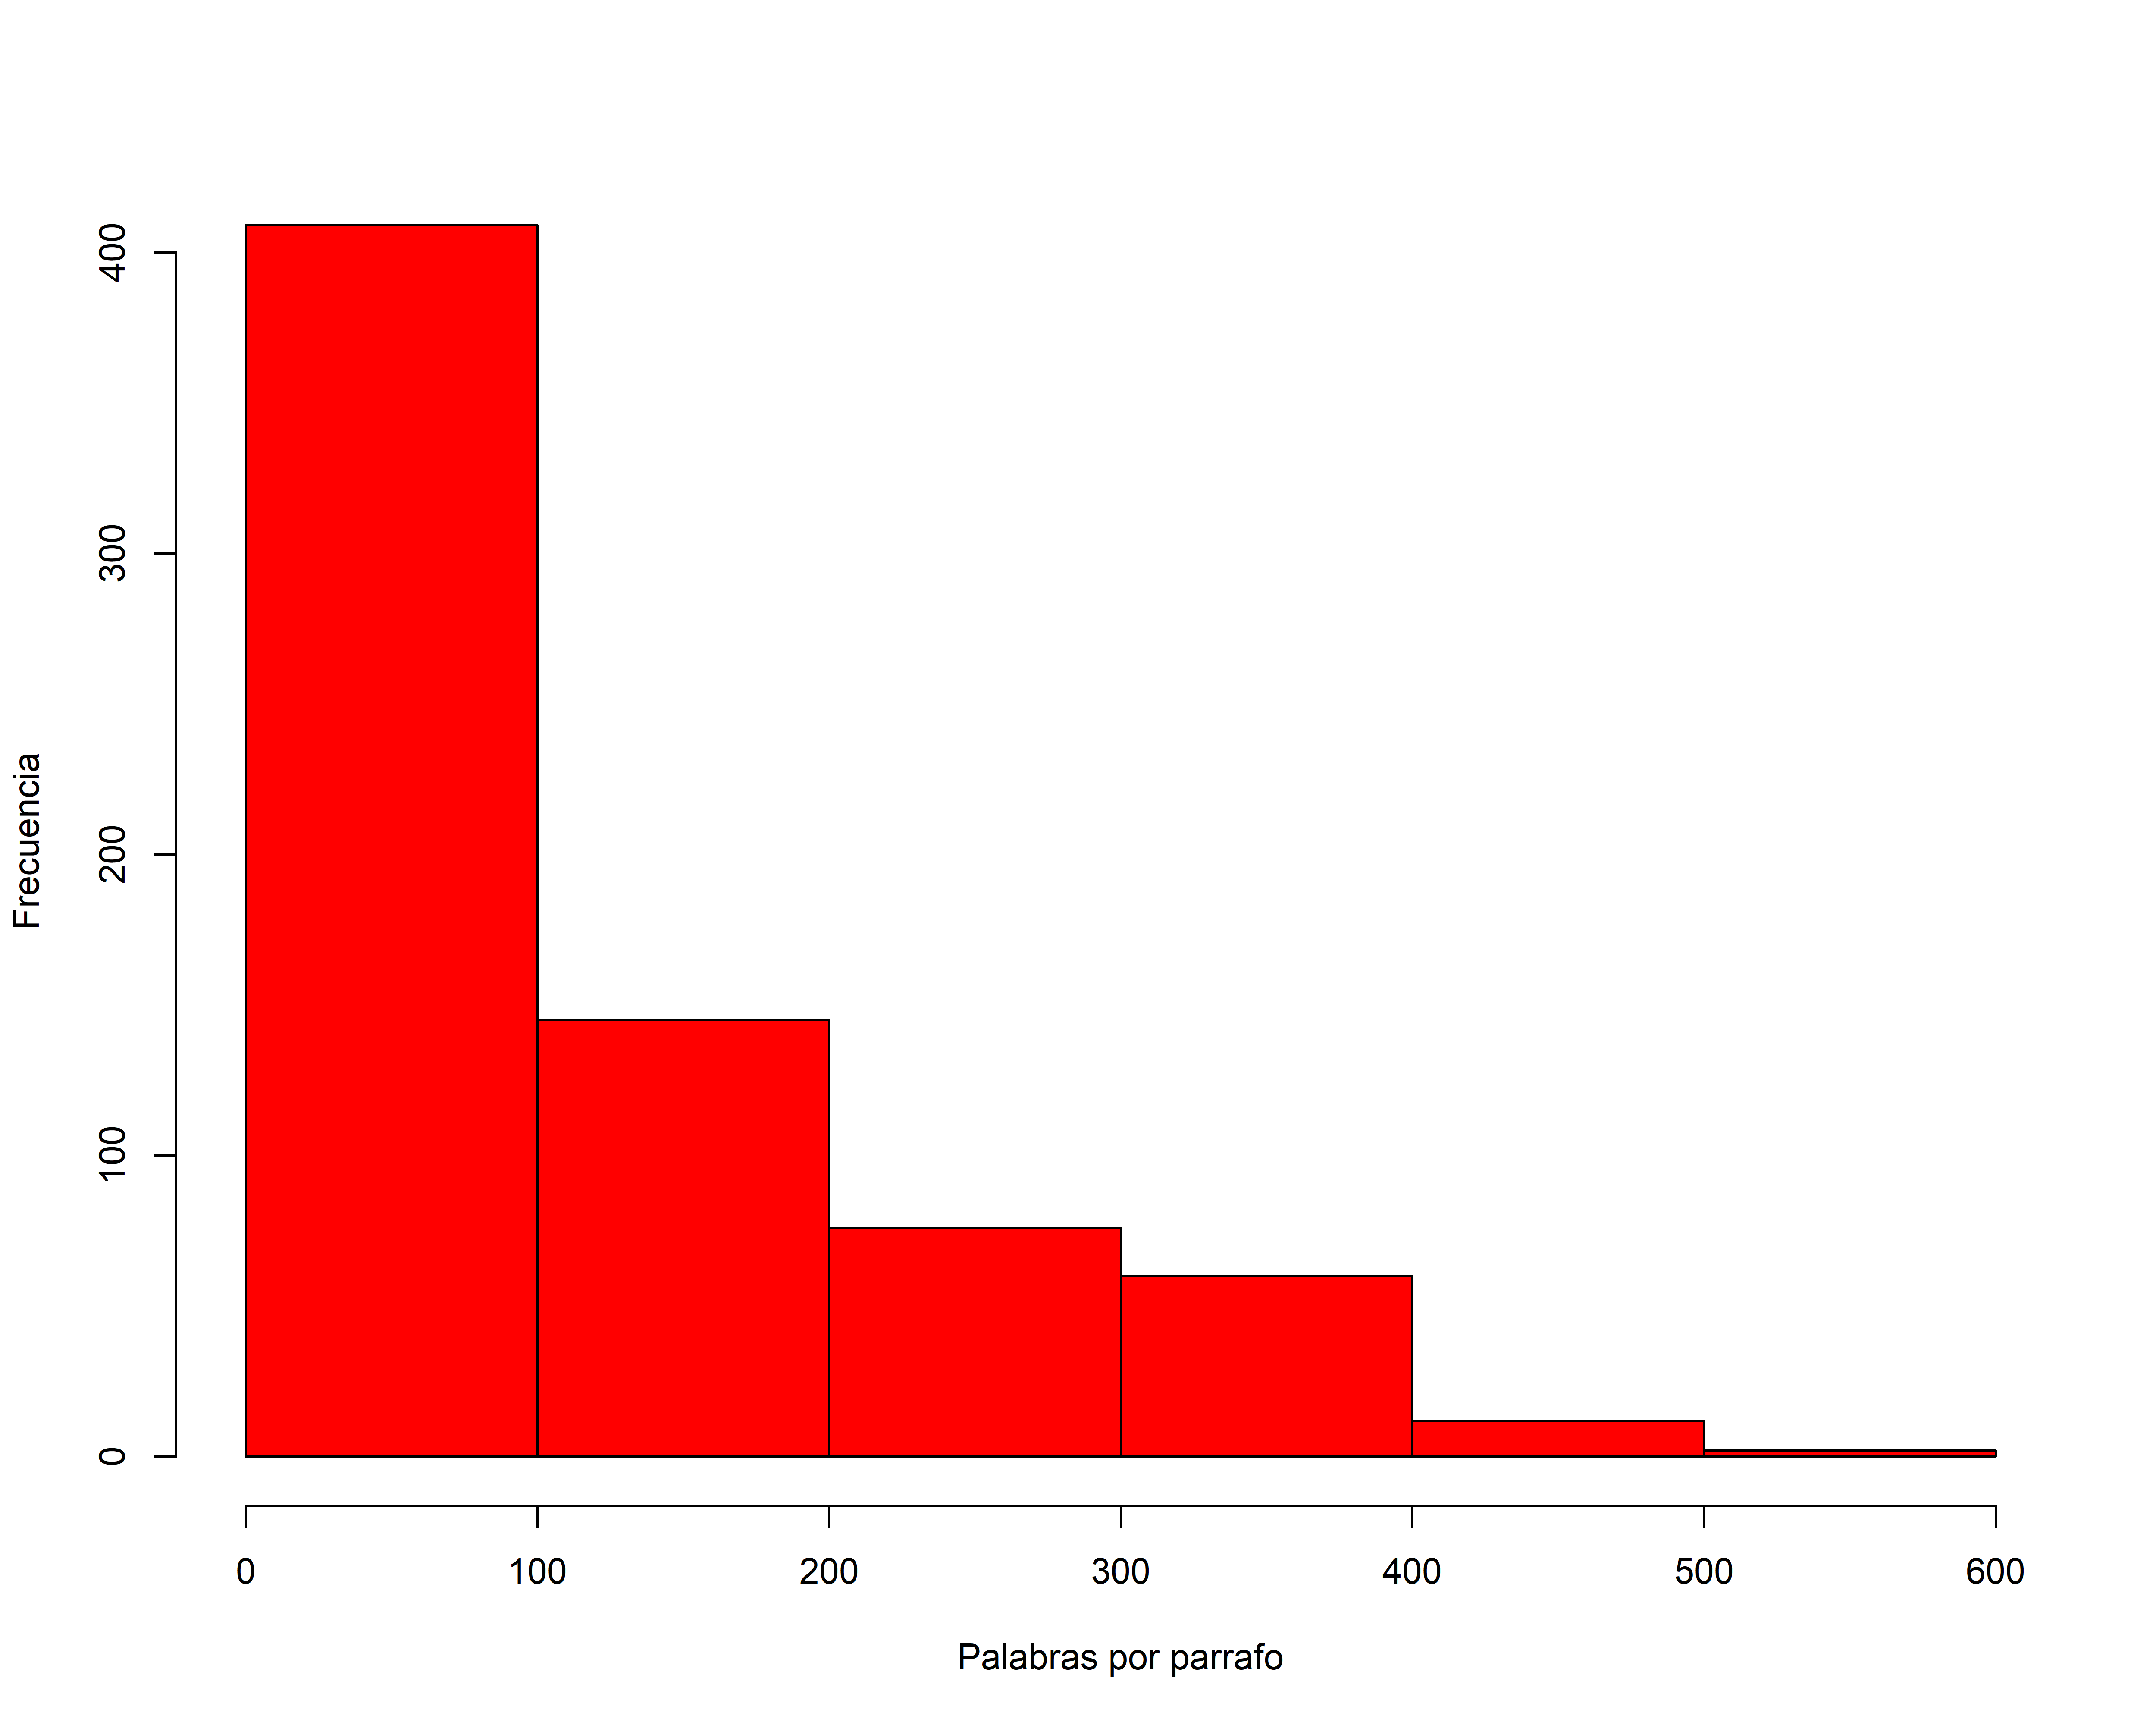
\includegraphics[scale=0.5]{Figures/palParrafos.png}
\caption{Distribución de la cantidad de palabras en cada párrafo (en párrafos con más de 9 palabras)}
\label{palParrafos}
\end{figure}

\section{Simulación de distribuciones}
Con el fin de simular las distribuciones geométrica, binomial y binomial negativa, se escogieron como criterios algunas características relevantes del análisis estadístico realizado anteriormente, como por ejemplo la letra y palabra con mayor frecuencia.

Para la distribución geométrica, se consideró el criterio de cuantos caracteres alfanuméricos hay antes de encontrar la letra con mayor frecuencia en todo el texto, en este caso, el éxito será encontrar la letra \texttt{e}. En la figura ref{\letraE} se puede observar como el criterio seleccionado sigue una distribución geométrica.


\begin{figure}
\centering
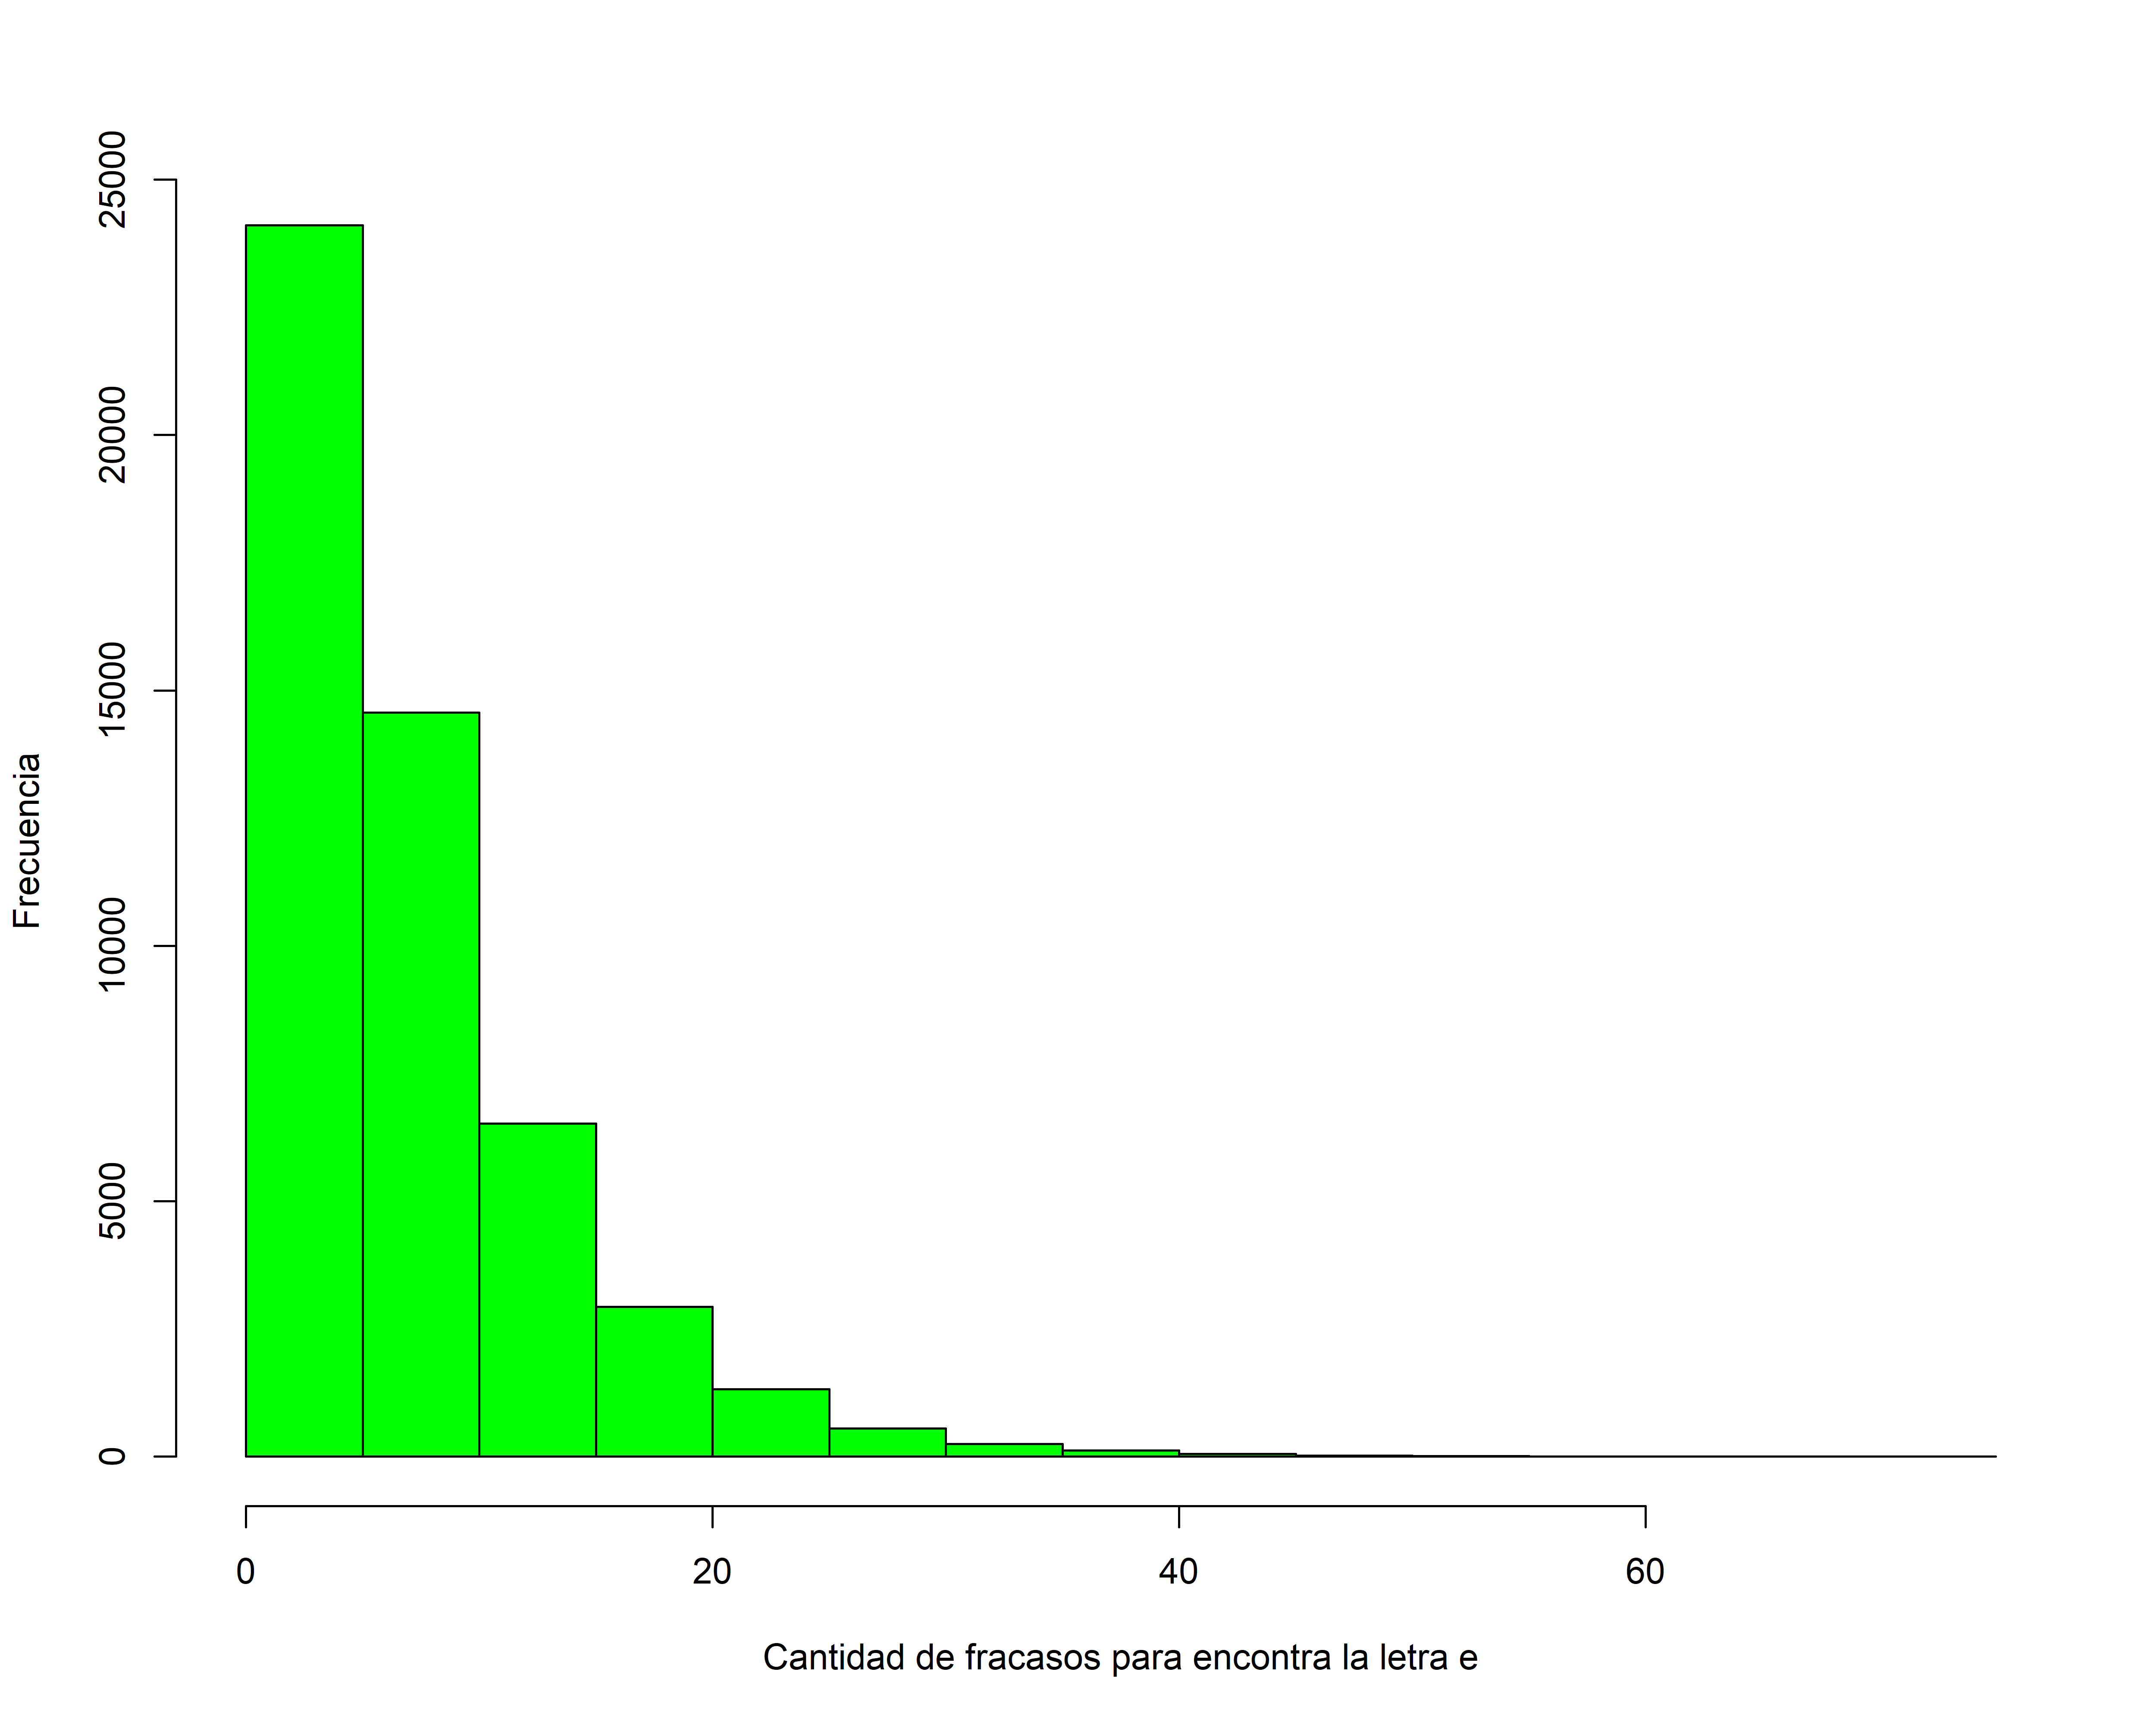
\includegraphics[scale=0.5]{Figures/letraE.png}
\caption{Distribución geométrica usando como éxito la letra con mayor frecuencia en el libro}
\label{letraE}
\end{figure}

Para la distribución binomial se consideró que las repeticiones se formarían con los párrafos cuya longitud de palabras es igual a $9$, ya que son los más frecuentes y como longitud de palabra igual a $2$, ya que es la menor cantidad de caracteres que pueda contener este tipo de párrafos. Con esta simulación se pretende encontrar cuantas palabras con la longitud dada (éxitos) se encuentran en los párrafos con las características mencionadas anteriormente. En la figura \ref{cantPalabras} se puede observar como el criterio seleccionado sigue una distribución binomial. Cabe mencionar que como la muestra es muy pequeña, son muy pocos los datos obtenidos.


\begin{figure}
\centering
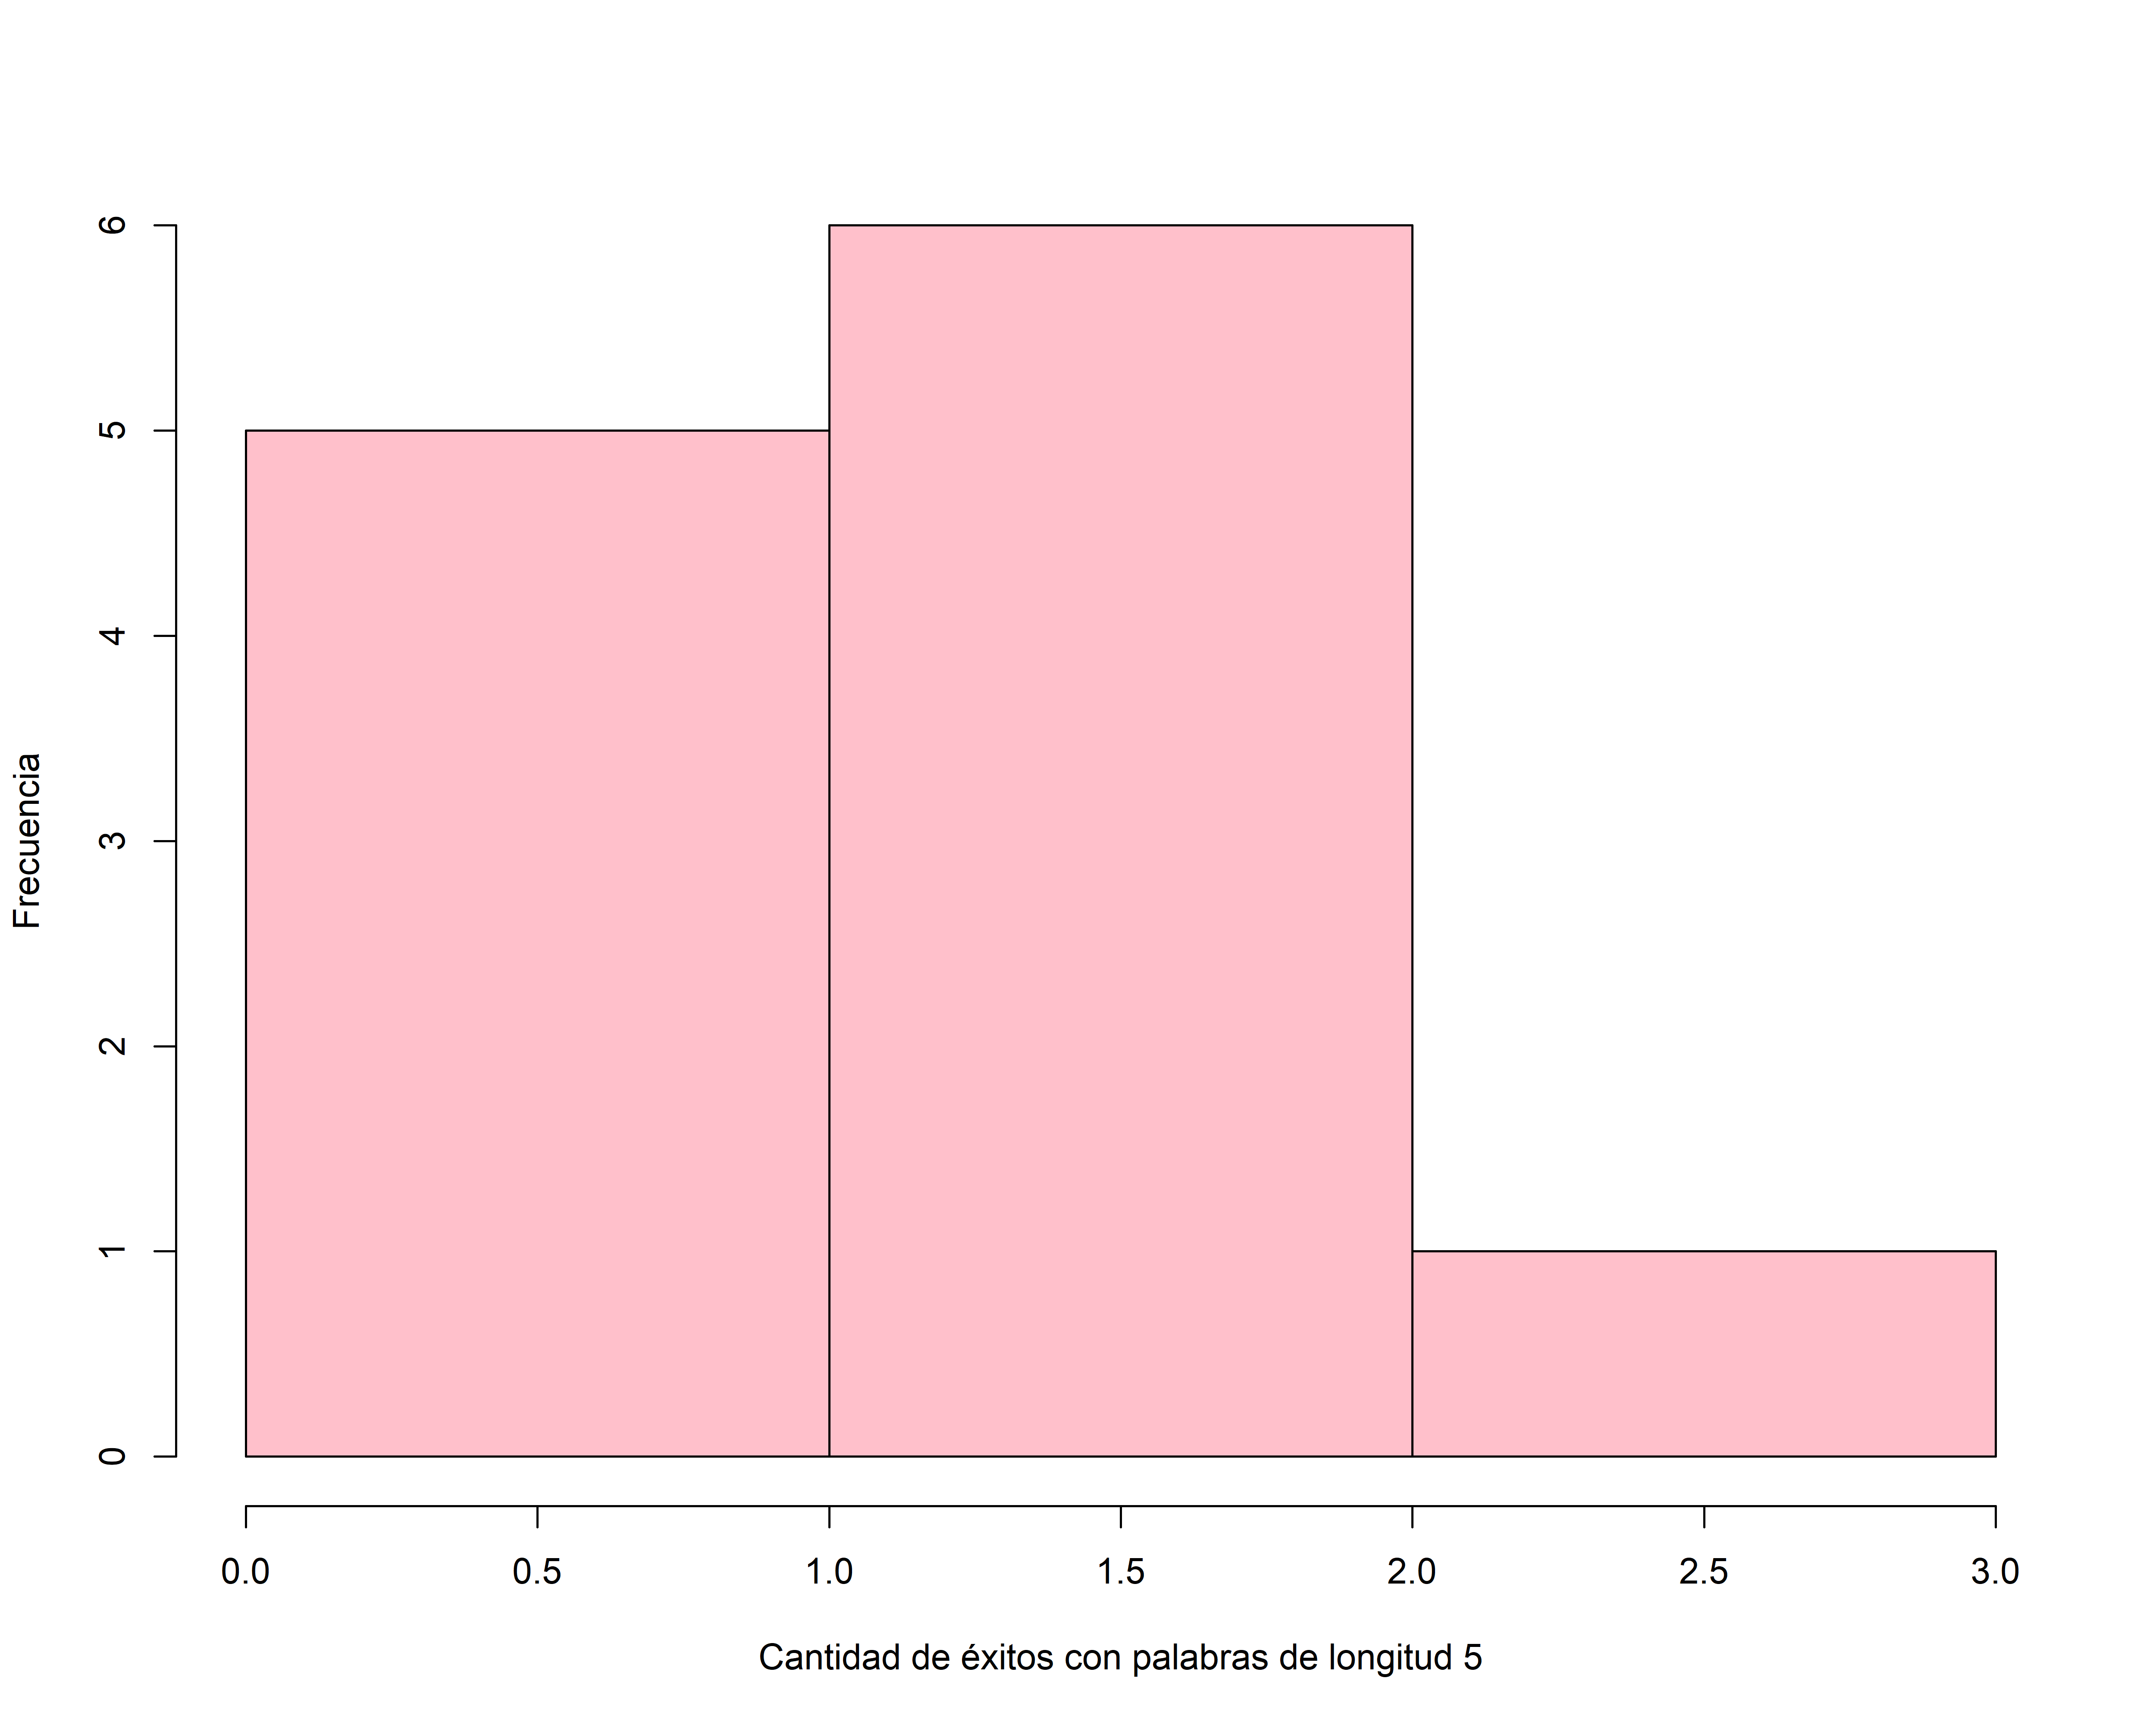
\includegraphics[scale=0.5]{Figures/cantPalabras.png}
\caption{Distribución binomial usando como éxito la cantidad de palabras con una deterinada longitud}
\label{cantPalabras}
\end{figure}

Finalmente, para la distribución binomial negativa, se consideró hallar la cantidad de intentos para completar $5$ éxitos en todo el libro, se considera un éxito cuando la letra \texttt{h} tiene seguida la letra \texttt{e}. Se contempló este criterio ya que la palabra y artículo más frecuente es \texttt{hester} y \texttt{the}, respectivamente. En la figura \ref{he} se puede observar como el criterio seleccionado sigue una distribución binomial negativa.


\begin{figure}
\centering
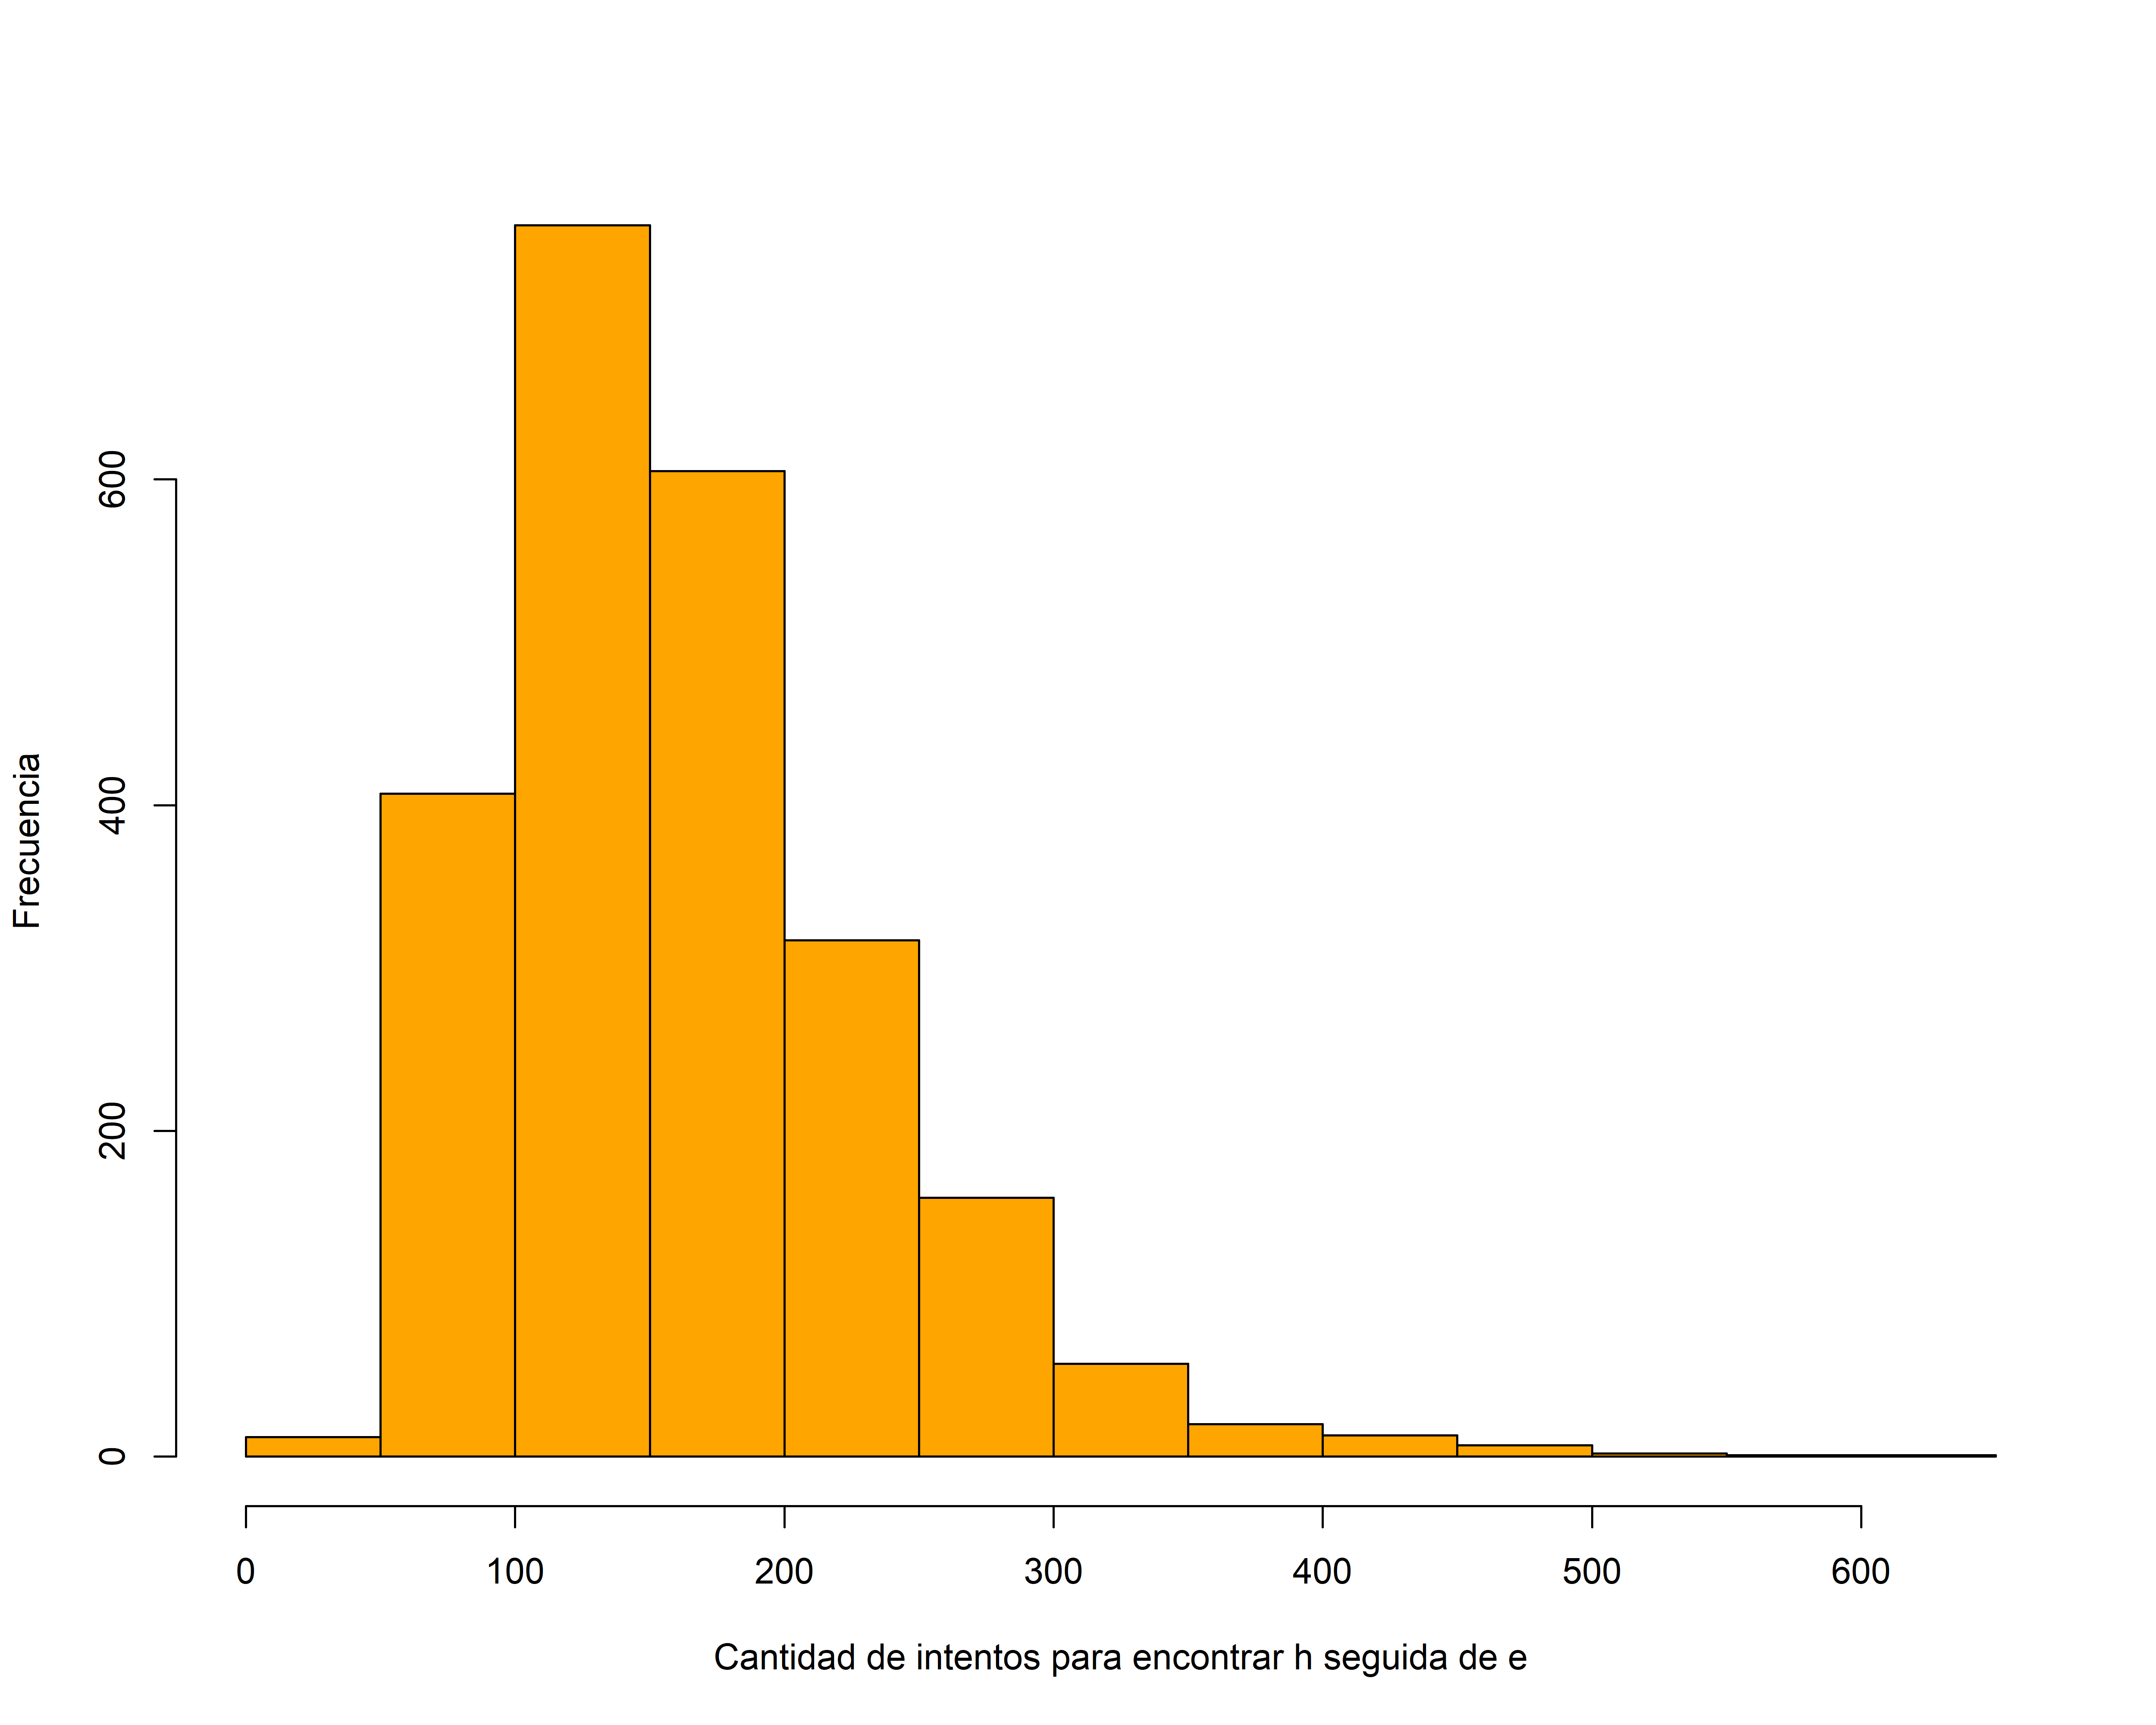
\includegraphics[scale=0.5]{Figures/he.png}
\caption{Distribución binomial negativa}
\label{he}
\end{figure}


\bibliography{refProbabilidad}
\bibliographystyle{plain}

\end{document}
